\documentclass[utf8]{beamer}
\mode<presentation>
\usepackage{listings}
\usepackage{helvet}
\usetheme{Warsaw}
\usecolortheme{whale}
\usefonttheme[onlylarge]{structuresmallcapsserif}
\usefonttheme[onlysmall]{structurebold}

\setbeamercovered{dynamic}
\setbeameroption{show notes}

\begin{document}
\title{Scaling Erlang Web Applications}
\subtitle{100 to 100K users at one web server}
\author{Fernando Benavides (\textit{@elbrujohalcon})}
\institute{Inaka Labs}
\date{\today}
\logo{
\includegraphics[height=0.5cm]{img/inaka_leaf_logo.png}}

\lstset{% general command to set parameter(s)
		basicstyle=\ttfamily\tiny, % print whole listing small
		keywordstyle=\color{black}\bfseries,
		identifierstyle=, % nothing happens
		stringstyle=\ttfamily, % typewriter type for strings
		showstringspaces=false} % no special string spaces

\lstset{language=erlang}
\defverbatim[colored]\startchild{%
\begin{lstlisting}[frame=single]
      supervisor:start_child(
      	list_to_atom("module-name_" ++
				integer_to_list(random:uniform(#ofSupervisors))).
\end{lstlisting}
}

\frame{\titlepage} 

\begin{frame}{Hello World!}
	\begin{itemize}
		\item<+-> I'm a developer since I was 10
		\item<+-> I'm an Erlang developer since 2008
	\end{itemize}
	\only<1>{
		\begin{center}
			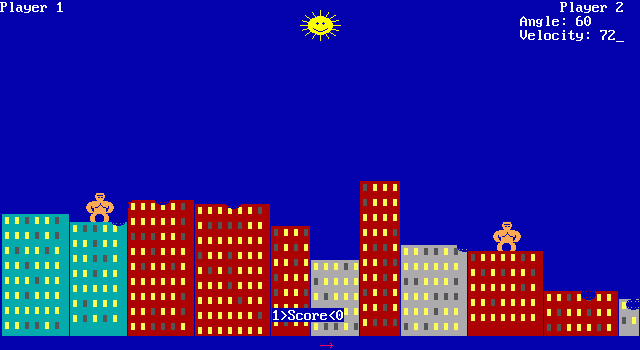
\includegraphics[width=.75\textwidth]{img/Gorillas.png}
		\end{center}
	}
	\only<2>{
		\begin{center}
			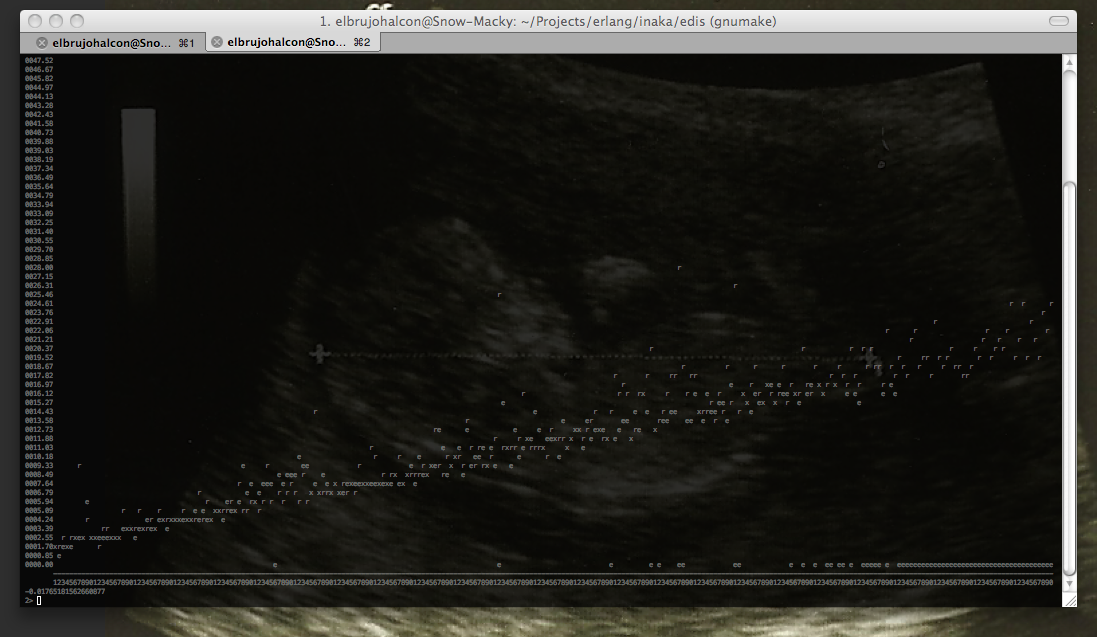
\includegraphics[width=.75\textwidth]{img/ErlangASCIIArt.png}
		\end{center}
	}
\end{frame}
\begin{frame}{Hello World!}
	\begin{itemize}
		\item<+-> I've built several dynamic web servers
			\begin{itemize}
				\item<+-> Many of them with real-time updates
				\item<+-> Most of them with high scale requirements
			\end{itemize}
		\item<+-> I'll show you how I make them scale
	\end{itemize}
\end{frame}

\section{Introduction}
\subsection{Description}
\begin{frame}{Introduction}
	We will work on the scalability of a \emph{web} project \pause that has an \emph{HTTP API} \pause and a component that keeps clients \emph{connected} to the server \pause for \emph{long periods} of time.\\
\pause Examples:
	\begin{itemize}
		\item<+-> Social sites
		\item<+-> Chat sites
		\item<+-> Sports sites
	\end{itemize}
\end{frame}

\subsection{Scope}
\begin{frame}{Scope}
	\emph{We will try to improve the way we use}
	\begin{itemize}
		\item OTP behaviours
		\item TCP and HTTP connections
		\item Underlaying system configurations
	\end{itemize}
	\pause
	\emph{We will \textbf{not} deal with}
	\begin{itemize}
		\item Multiple machines/nodes
		\item Database choices and/or implementations
	\end{itemize}
\end{frame}

\section{Match Stream}
\subsection{Idea}
\begin{frame}[t]{Match Stream}{General Idea}
	\only<1>{
		\emph{A soccer match is played at some stadium}
		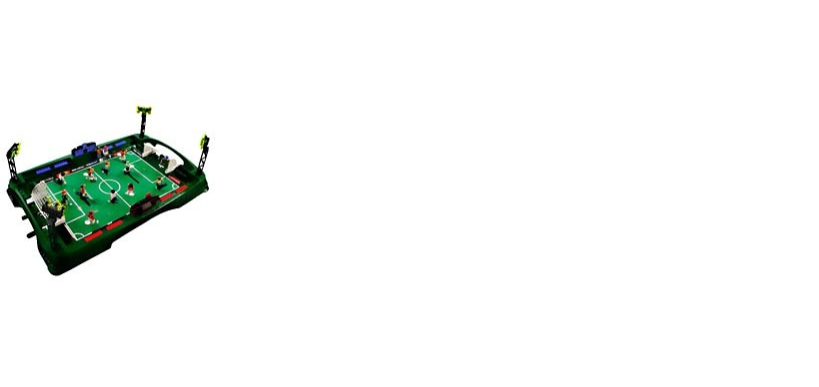
\includegraphics[width=\textwidth]{img/overview-1.png}}
	\only<2>{
		\emph{Soccer fans are connected to the internet in their offices}
		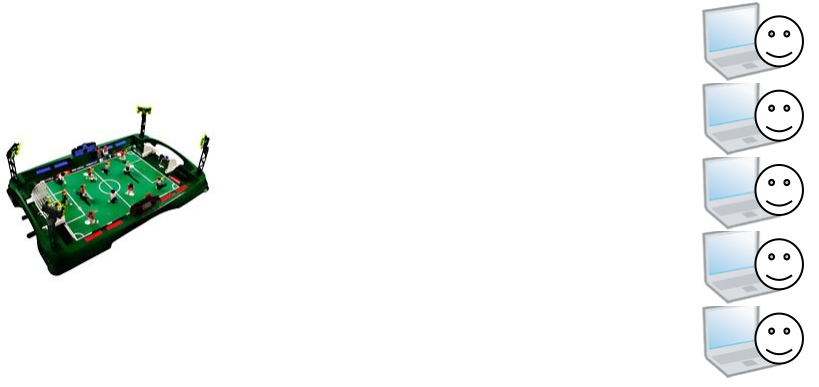
\includegraphics[width=\textwidth]{img/overview-2.png}}
	\only<3>{
		\emph{A reporter is at the stadium with his device}
		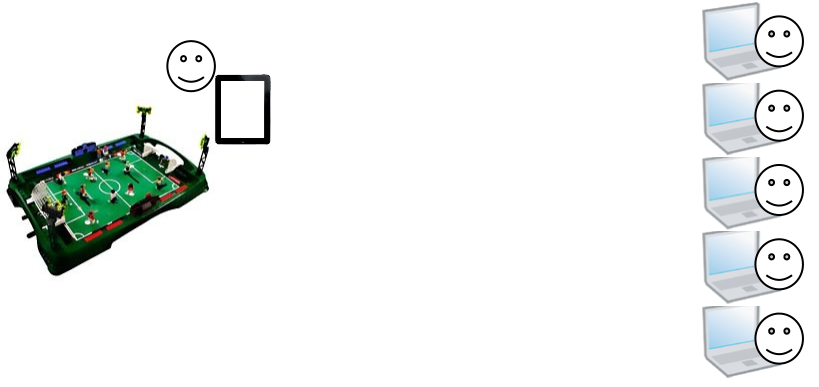
\includegraphics[width=\textwidth]{img/overview-3.png}}
	\only<4>{
		\emph{\textsc{MatchStream} \textbf{connects} them in \textbf{real time}}
		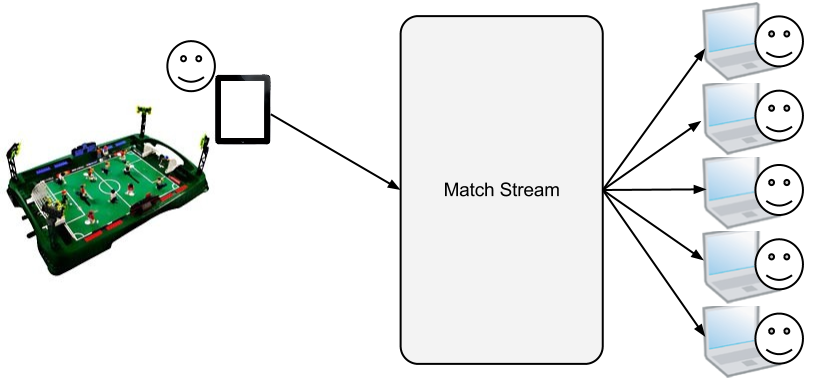
\includegraphics[width=\textwidth]{img/overview-4.png}}
\end{frame}
\begin{frame}{Match Stream}{Requirements}
	\textsc{System Challenges}
	\begin{itemize}
		\item<+-> Tons of concurrent users
		\item<+-> Two-hour-long bursts of connections followed by long periods of inactivity
		\item<+-> Real-time updates
	\end{itemize}
	\onslide<+->Erlang seems to be \textbf{the right fit for this}
\end{frame}

\subsection{Design}
\begin{frame}{Match Stream}{General Design}
	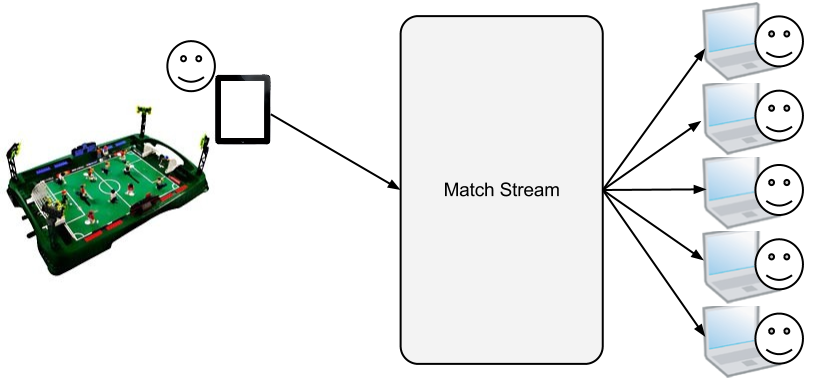
\includegraphics[width=\textwidth]{img/MatchStream.png}
\end{frame}
\begin{frame}[t]{Match Stream}{Architecture}
	\only<1>{
		\begin{center}
			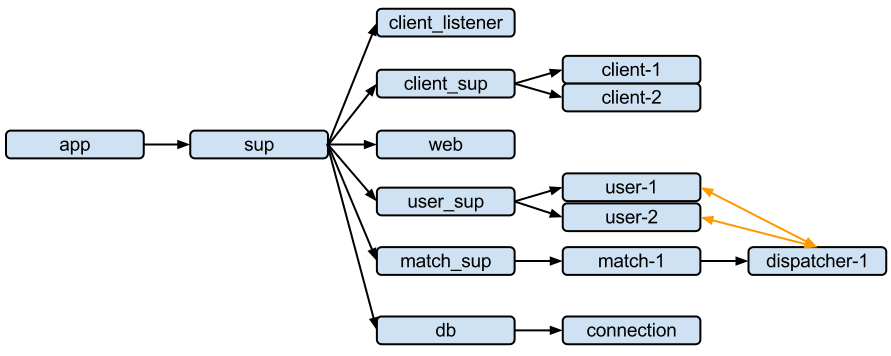
\includegraphics[width=\textwidth]{img/architecture-1.png}
		\end{center}}
	\only<2>{
		\begin{center}
			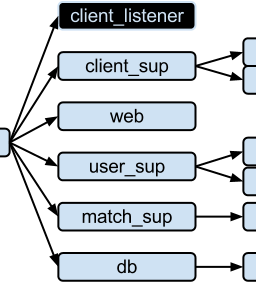
\includegraphics[width=\textwidth]{img/architecture-1-1.png}
		\end{center}
		\begin{description}
			\item[client\_listener]
				\texttt{gen\_server}. Listens on a TCP port to receive client connections
		\end{description}}
	\only<3>{
		\begin{center}
			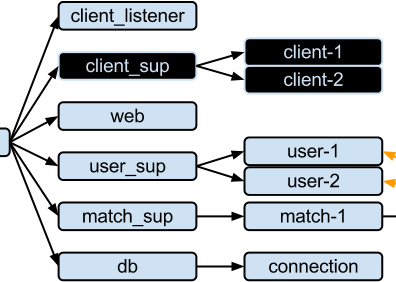
\includegraphics[width=\textwidth]{img/architecture-1-2.png}
		\end{center}
		\begin{description}
			\item[client\_sup]
				\texttt{supervisor}. Supervises connection processes
			\item[client]
				\texttt{gen\_fsm}. Handles a TCP connection
		\end{description}}
	\only<4>{
		\begin{center}
			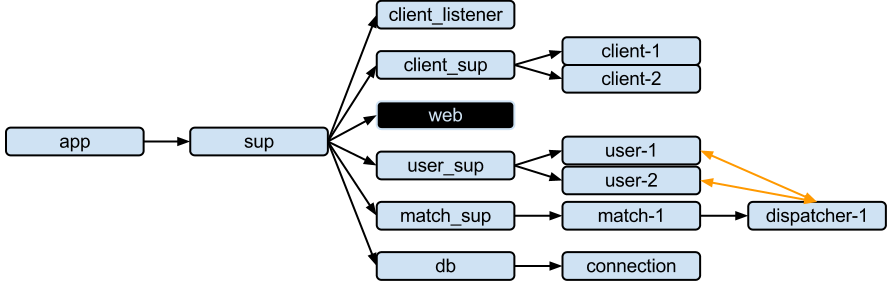
\includegraphics[width=\textwidth]{img/architecture-1-3.png}
		\end{center}
		\begin{description}
			\item[web]
				\texttt{mochiweb server}. Listens for HTTP API calls
		\end{description}}
	\only<5>{
		\begin{center}
			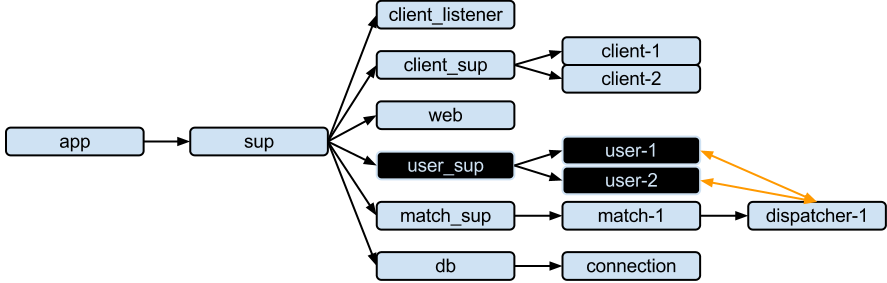
\includegraphics[width=\textwidth]{img/architecture-1-4.png}
		\end{center}
		\begin{description}
			\item[user\_sup]
				\texttt{supervisor}. Supervises user processes
			\item[user]
				\texttt{gen\_server}. Subscribes to match dispatchers and sends events to clients
		\end{description}}
	\only<6>{
		\begin{center}
			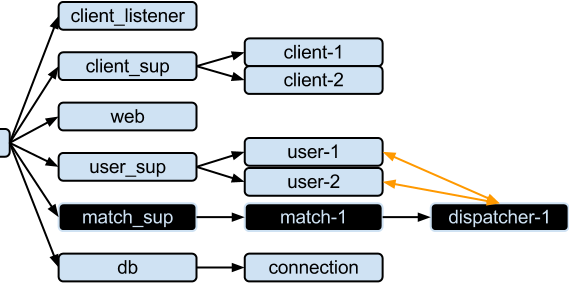
\includegraphics[width=\textwidth]{img/architecture-1-5.png}
		\end{center}
		\begin{description}
			\item[match\_sup]
				\texttt{supervisor}. Supervises match processes
			\item[match]
				\texttt{gen\_server}. Listens to match events, stores them
			\item[dispatcher]
				\texttt{gen\_event dispatcher}. Delivers match events
		\end{description}}
	\only<7>{
		\begin{center}
			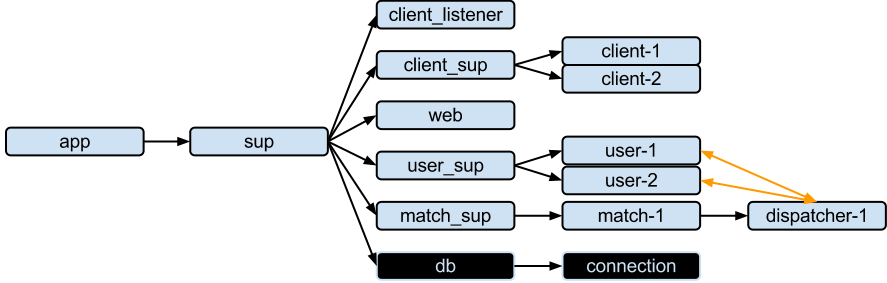
\includegraphics[width=\textwidth]{img/architecture-1-6.png}
		\end{center}
		\begin{description}
			\item[db]
				\texttt{gen\_server}. Processes database operations
			\item[connection]
				\texttt{erldis client}. Handles the connection to the database
		\end{description}}
\end{frame}

\section{Scaling}
\begin{frame}{Lesson Learned}
	\begin{center}
		\huge \emph{Using Erlang to build your system is \textbf{not enough} to ensure \textbf{scalability}}
	\end{center}
\end{frame}

\subsection{Stage 1: The Original System}
\begin{frame}{Stage 1}{Testing the system as it is}
	\textsc{Goals}
	\begin{itemize}
		\item Find how much the system can handle
	\end{itemize}
	\pause
	\textsc{Steps}
	\begin{itemize}
		\item Create automated testers
		\item Start the system on a \emph{clean} machine
		\item Test repeatedly adjusting the number of connections
		\item Have a human trying the system himself
	\end{itemize}
\end{frame}
\begin{frame}{Stage 1}{Results}
	\begin{columns}
		\column{.66\textwidth}
			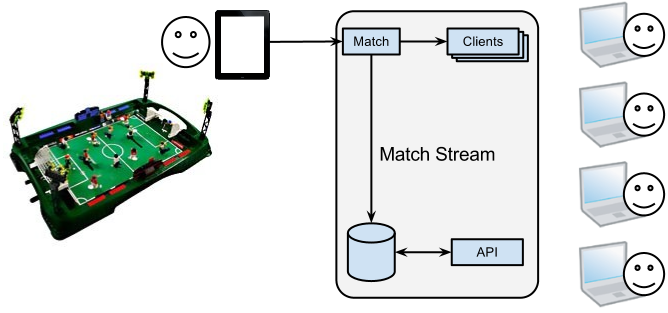
\includegraphics[top=-1,width=\textwidth]{img/results-1.png}
		\column{.33\textwidth}
			\begin{itemize}
				\item \textbf{\Large 1024} users
				\item \textbf{\Large 4} at a time
				\item \textbf{\Large 10s} ART
			\end{itemize}
	\end{columns}
\end{frame}

\subsection{Stage 2: OS Tuning}
\begin{frame}{Stage 2}{Improving the Environment}
	\textsc{Goals}
	\begin{itemize}
		\item Improve the system environment without altering the code
	\end{itemize}
	\pause
	\textsc{Settings to Tune Up}
	\begin{itemize}
		\item<+-> Concurrent TCP connections
		\item<+-> Open files limit
		\item<+-> TCP backlog size
		\item<+-> TCP memory allocation
		\item<+-> Erlang VM startup parameters
	\end{itemize}
\end{frame}
\begin{frame}{Stage 2}{Results}
	\begin{columns}
		\column{.66\textwidth}
			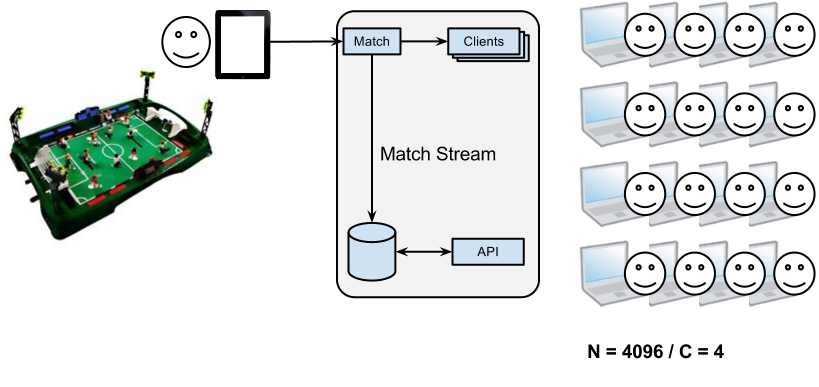
\includegraphics[top=-1,width=\textwidth]{img/MatchStream-2.png}
		\column{.33\textwidth}
			\begin{itemize}
				\item \textbf{\Large 4096} users
				\item \textbf{\Large 4} at a time
				\item \textbf{\Large 9s} ART
			\end{itemize}
	\end{columns}
\end{frame}

\subsection{Stage 3: Erlang Tuning}
\begin{frame}{Stage 3}{Improving Match Stream}
	\textsc{Goals}
	\begin{itemize}
		\item Tune up the system for \alert{one node}
	\end{itemize}
	\pause
	\textsc{Steps}
	\begin{itemize}
		\item Find a problem
		\item Fix it using the list of \emph{Tips and Tricks}
		\item If not there, add it
		\item Repeat from \alert{Stage 1}
	\end{itemize}
\end{frame}

\subsubsection{TCP Tuning}
\begin{frame}{Stage 3.1}{Connection Tweaks}
	\begin{description}
		\item<+->[Backlog]\ \\
			\begin{itemize}
				\item Allow more concurrent connections
				\item Don't forget TCP tuning your HTTP server
			\end{itemize}
		\item<+->[Connections]\ \\
			\begin{itemize}
				\item Don't use just one of them
				\item Check inbound and outbound connections
			\end{itemize}
	\end{description}
\end{frame}
\begin{frame}{Stage 3.1}{Connection Tweaks}
	\textsc{System Architecture}
	\begin{center}
		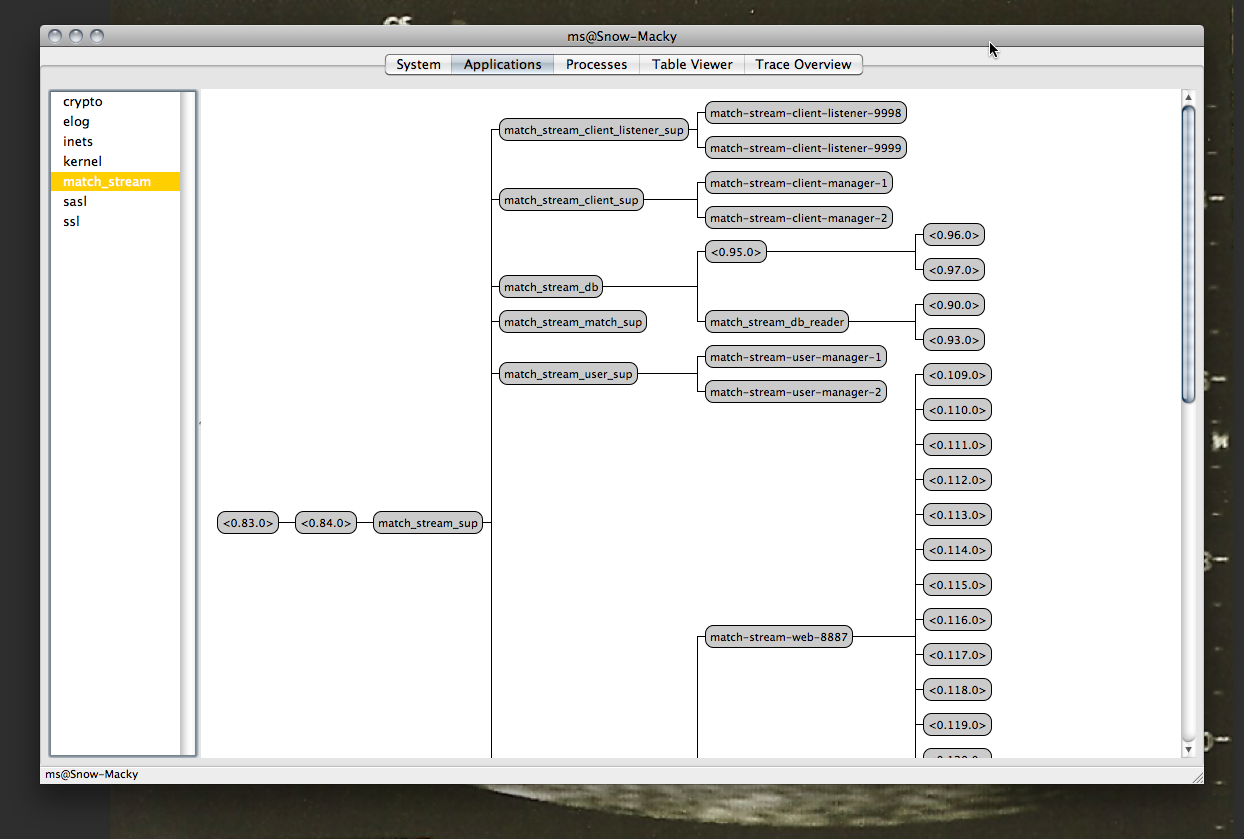
\includegraphics[height=.75\textheight]{img/running-late.png}
	\end{center}
\end{frame}
\begin{frame}{Stage 3.1}{Results}
	\begin{columns}
		\column{.66\textwidth}
			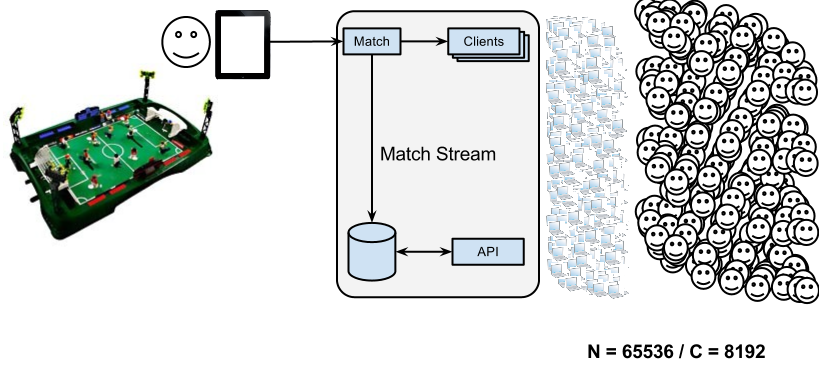
\includegraphics[top=-1,width=\textwidth]{img/MatchStream-3.png}
		\column{.33\textwidth}
			\begin{itemize}
				\item \textbf{\Large 8192} users
				\item \textbf{\Large 256} at a time
				\item \textbf{\Large 16s} ART
			\end{itemize}
	\end{columns}
\end{frame}

\subsubsection{OTP}
\begin{frame}{Stage 3.2}{gen\textunderscore event}
	\begin{description}
		\item<+->[sup\textunderscore handler]\ \\
			\begin{itemize}
				\item Don't use it
				\item Monitor the processes instead
			\end{itemize}
		\item<+->[Long Delivery Queues]\ \\
			\begin{itemize}
				\item Use \emph{repeaters}
			\end{itemize}
	\end{description}
\end{frame}
\begin{frame}{Stage 3.2}{gen\textunderscore event}
	\textsc{System Architecture}
	\begin{center}
		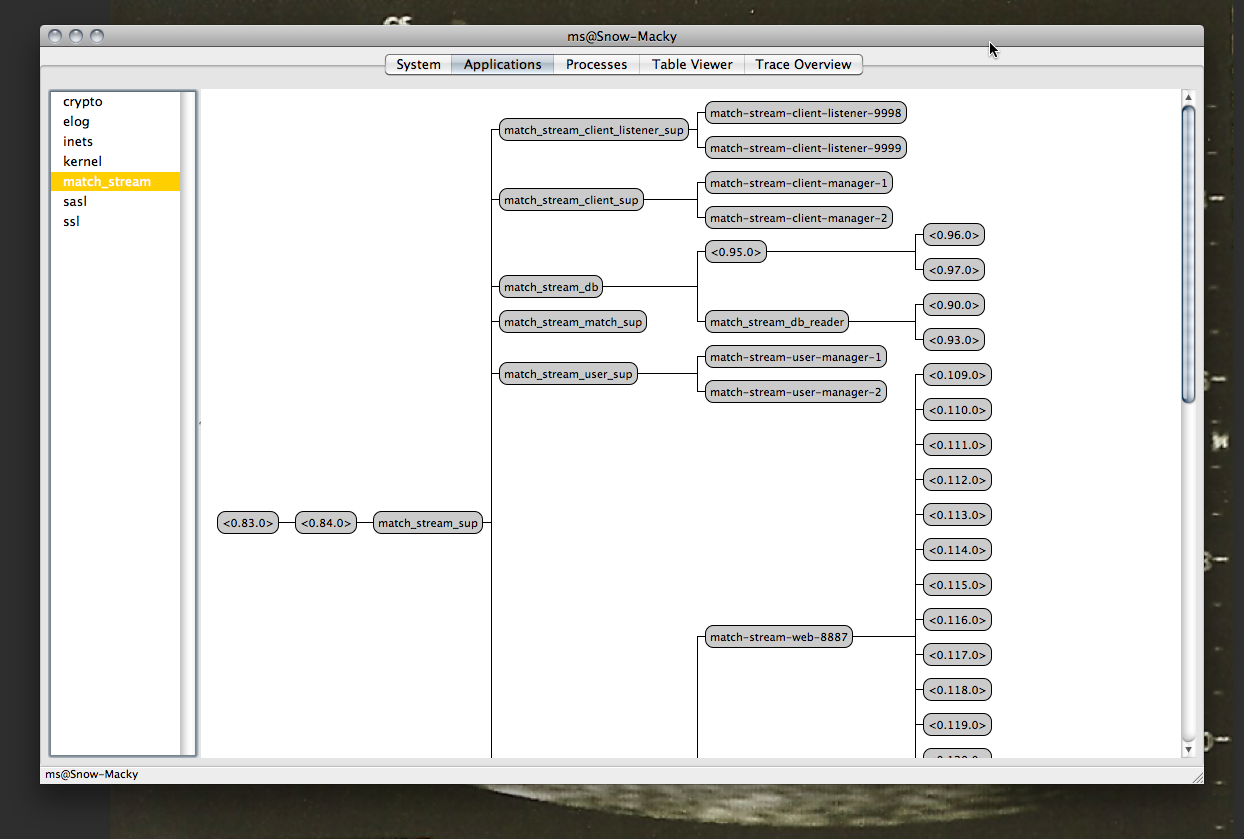
\includegraphics[height=.75\textheight]{img/running-late.png}
	\end{center}
\end{frame}
\begin{frame}{Stage 3.2}{Results}
	\begin{columns}
		\column{.66\textwidth}
			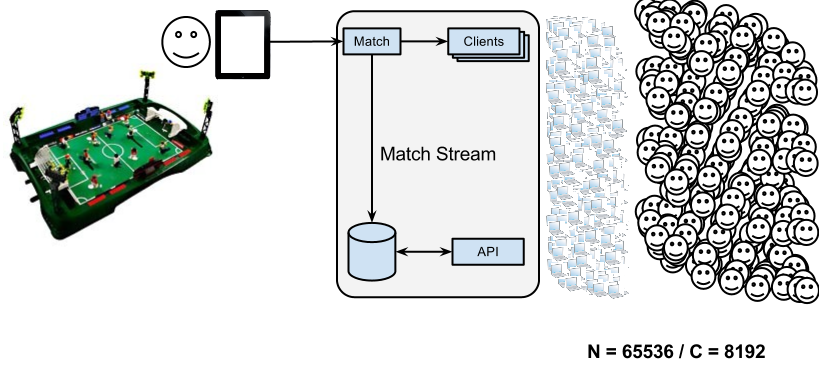
\includegraphics[top=-1,width=\textwidth]{img/MatchStream-3.png}
		\column{.33\textwidth}
			\begin{itemize}
				\item \textbf{\Large 8192} users
				\item \textbf{\Large 256} at a time
				\item \textbf{\Large 8s} ART
			\end{itemize}
	\end{columns}
\end{frame}
\begin{frame}{Stage 3.3}{gen\textunderscore server}
	\begin{description}
		\item<+->[Call Timeouts]\ \\
			Remember \texttt{gen\textunderscore server:reply/2}
		\item<+->[Memory Footprint]\ \\
			Remember \texttt{hibernate}
		\item<+->[Long \texttt{init/1}]\ \\
			Use $0$ timeout
	\end{description}
\end{frame}
\begin{frame}{Stage 3.3}{gen\textunderscore server}
	\textsc{System Architecture}
	\begin{center}
		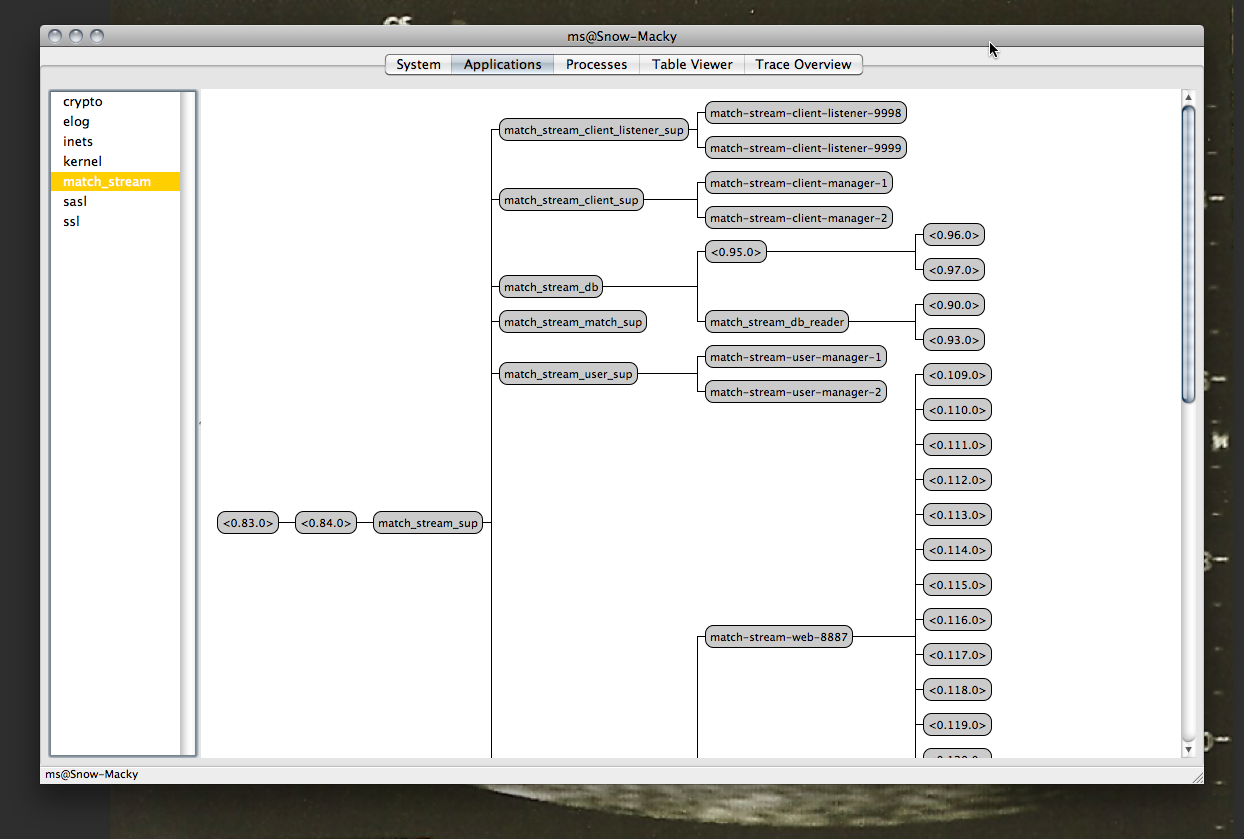
\includegraphics[height=.75\textheight]{img/running-late.png}
	\end{center}
\end{frame}
\begin{frame}{Stage 3.3}{Results}
	\begin{columns}
		\column{.66\textwidth}
			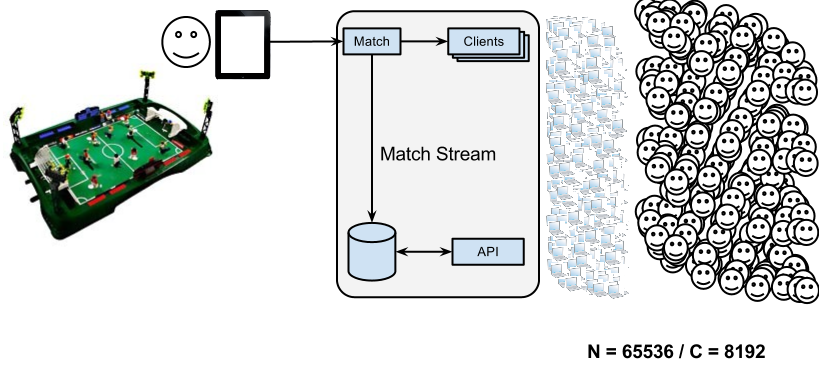
\includegraphics[top=-1,width=\textwidth]{img/MatchStream-3.png}
		\column{.33\textwidth}
			\begin{itemize}
				\item \textbf{\Large 32768} users
				\item \textbf{\Large 1024} at a time
				\item \textbf{\Large 1s} ART
			\end{itemize}
	\end{columns}
\end{frame}
\begin{frame}{Stage 3.4}{supervisors}
	\begin{itemize}
		\item Sometimes \texttt{simple\textunderscore one\textunderscore for\textunderscore one} supervisors get \alert{overburdened} because they have too many children
		\item Try a supervisor hierarchy with several managers below the main supervisor
		\item Turn \texttt{supervisor:start\textunderscore child/2} calls into something like
		\startchild
	\end{itemize}
\end{frame}
\begin{frame}{Stage 3.4}{supervisors}
	\textsc{System Architecture}
	\begin{center}
		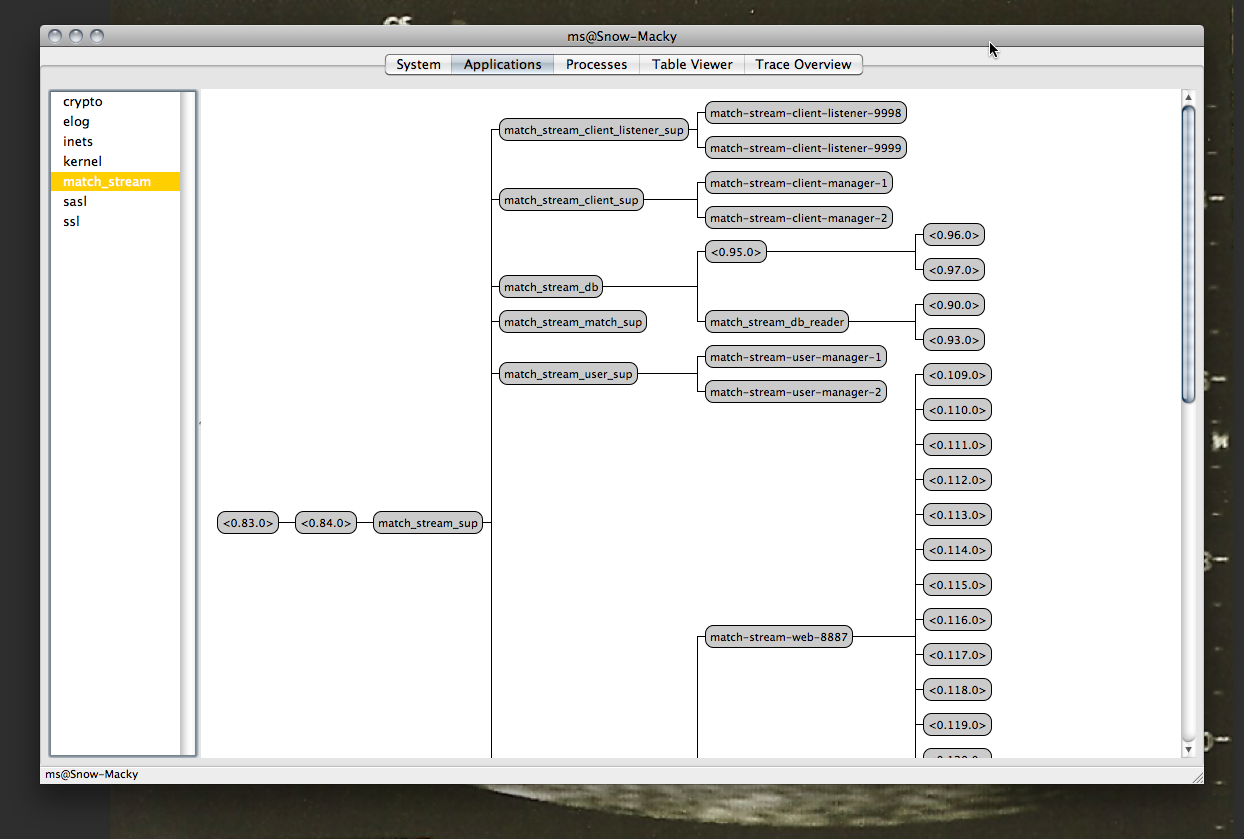
\includegraphics[height=.75\textheight]{img/running-late.png}
	\end{center}
\end{frame}
\begin{frame}{Stage 3.4}{Results}
	\begin{columns}
		\column{.66\textwidth}
			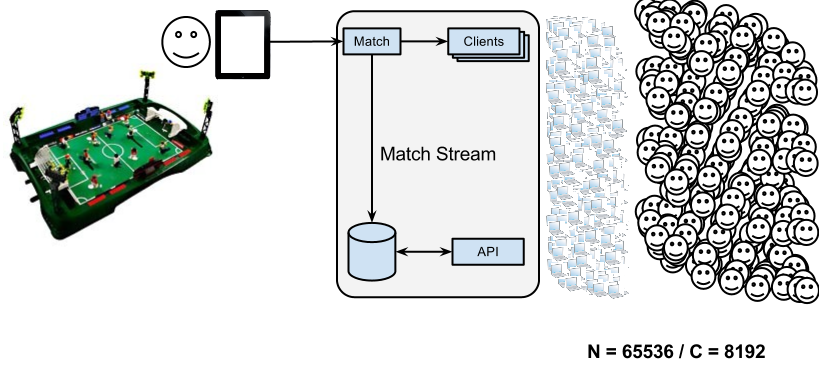
\includegraphics[top=-1,width=\textwidth]{img/MatchStream-3.png}
		\column{.33\textwidth}
			\begin{itemize}
				\item \textbf{\Large 65536} users
				\item \textbf{\Large 2048} at a time
				\item \textbf{\Large 1s} ART
			\end{itemize}
	\end{columns}
\end{frame}

\subsubsection{Other Stuff}
\begin{frame}{Stage 3.5}{Other Processes}
	\begin{description}
		\item<+->[Timers]\ \\
			\begin{itemize}
				\item Don't use the \texttt{timer} module
				\item Use \texttt{erlang:send\textunderscore after}
			\end{itemize}
		\item<+->[Logging]\ \\
			\begin{itemize}
				\item Don't log too much
				\item Use a good logging system
			\end{itemize}
		\item<+->[Registration]\ \\
			\begin{itemize}
				\item Sometimes it's better to register processes instead of keeping track of their pids manually
				\item You can always register processes \alert{both} locally and globally
			\end{itemize}
	\end{description}
\end{frame}
\begin{frame}{Stage 3.5}{Other Processes}
	\textsc{System Architecture}
	\begin{center}
		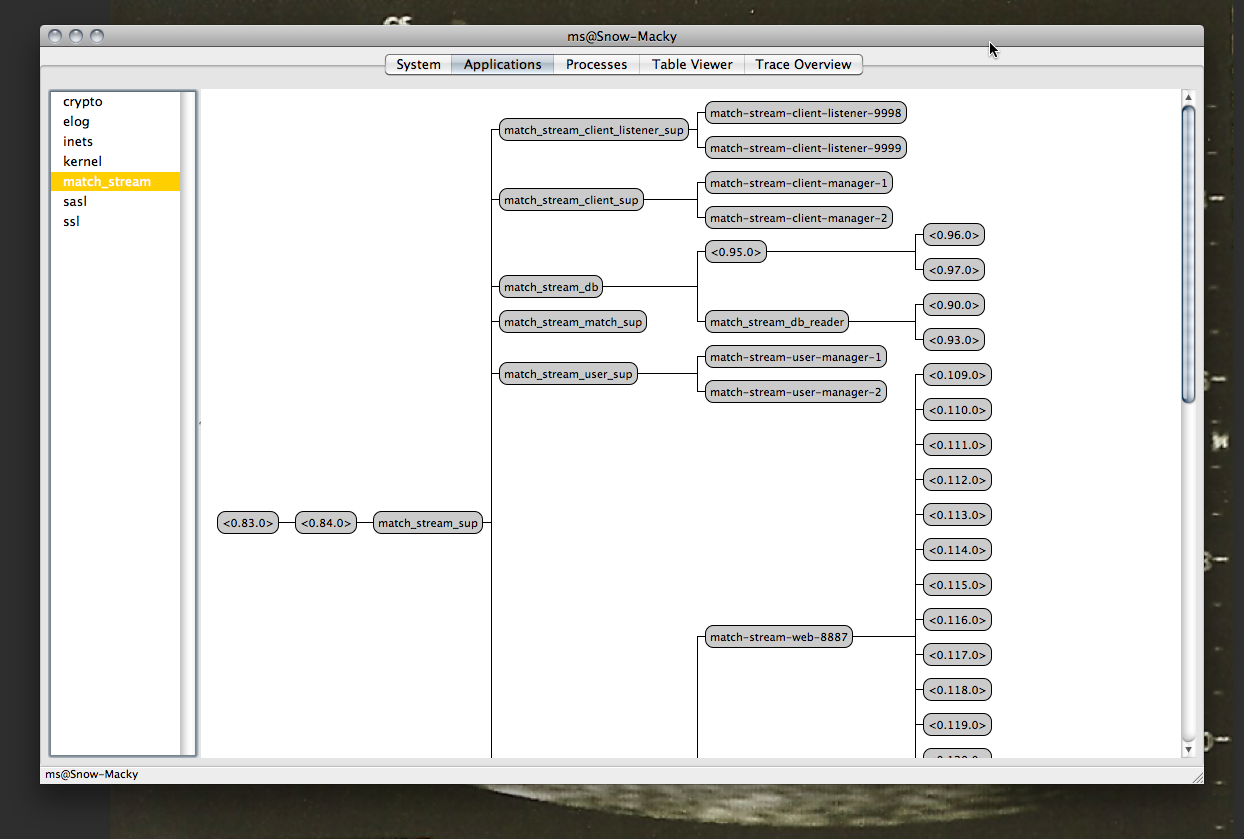
\includegraphics[height=.75\textheight]{img/running-late.png}
	\end{center}
\end{frame}
\begin{frame}{Stage 3.5}{Results}
	\begin{columns}
		\column{.66\textwidth}
			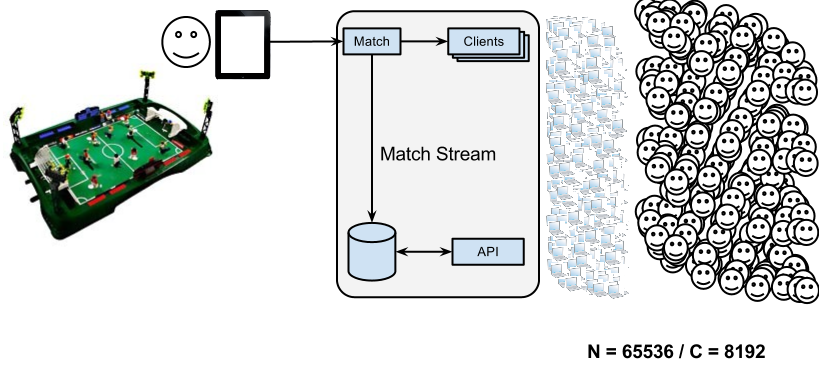
\includegraphics[top=-1,width=\textwidth]{img/MatchStream-3.png}
		\column{.33\textwidth}
			\begin{itemize}
				\item \textbf{\Large 65536} users
				\item \textbf{\Large 8192} at a time
				\item \textbf{\Large 10ms} ART
			\end{itemize}
	\end{columns}
\end{frame}

\subsection{Stage 4: Multi-Node Tuning}
\begin{frame}{Stage 4}{Adding Nodes}
	\textsc{Goals}
	\begin{itemize}
		\item Find the best system topology
	\end{itemize}
	\pause
	\textsc{Steps}
	\begin{itemize}
		\item Prepare the system to run in more than one node
		\item Decide if nodes should be connected or independent
		\item Decide if nodes should be on the same machine or not
	\end{itemize}
\end{frame}
\begin{frame}{Stage 4}{Adding Nodes}
	\textsc{System Architecture}
	\begin{center}
		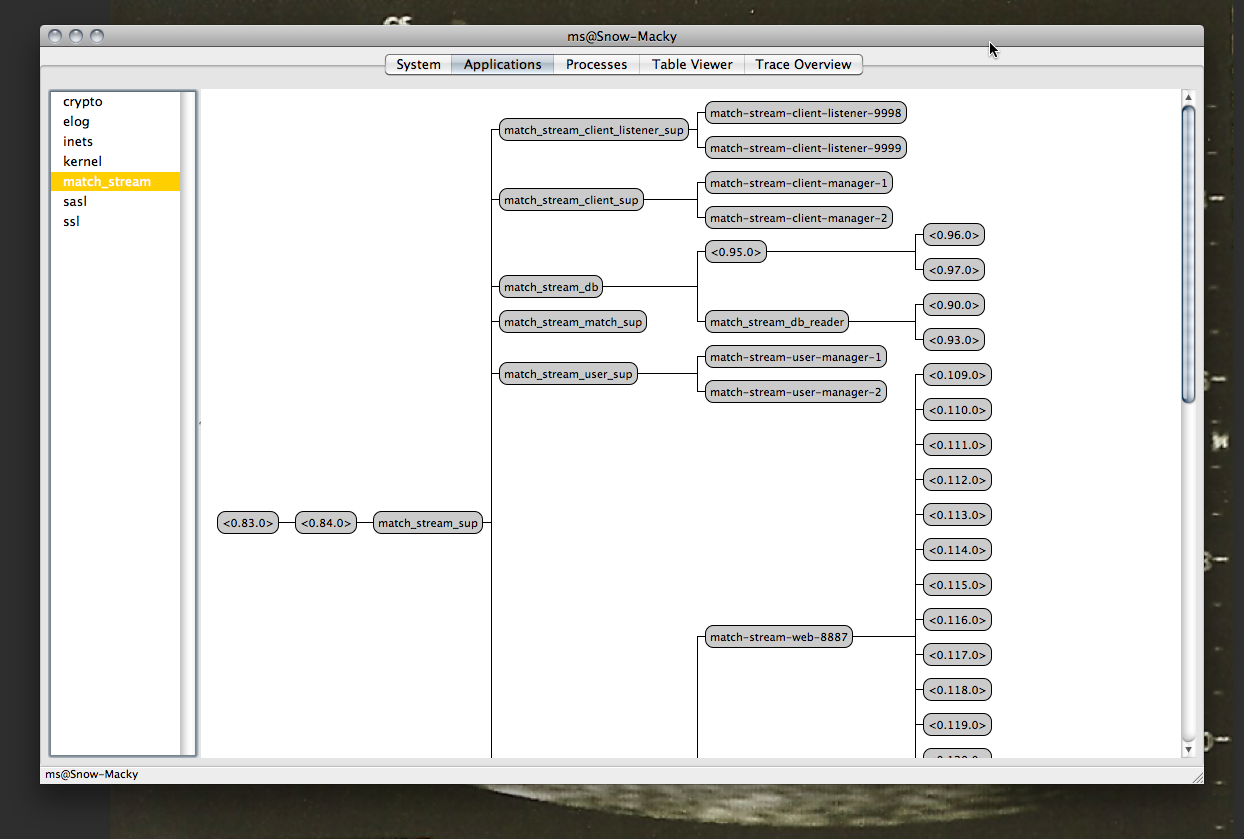
\includegraphics[height=.75\textheight]{img/running-late.png}
	\end{center}
\end{frame}
\begin{frame}{Stage 4}{Results}
	\begin{columns}
		\column{.66\textwidth}
			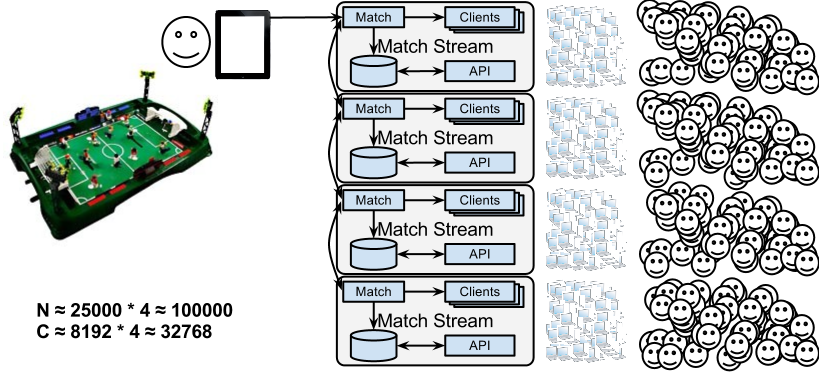
\includegraphics[top=-1,width=\textwidth]{img/MatchStream-4.png}
		\column{.33\textwidth}
			\begin{itemize}
				\item \textbf{\Large 100K} users
				\item \textbf{\Large 32768} at a time
				\item \textbf{\Large 10ms} ART
			\end{itemize}
	\end{columns}
\end{frame}

\section{Final Words}
\subsection{Summary}
\begin{frame}{Summary}
	\begin{itemize}
		\item<+-> This is an \alert{iterative} process
		\item<+-> It worked awesomely for us in both experimental and real-life systems
		\item<+-> It's no \alert{silver bullet}
		\item<+-> The list of \emph{Tips and Tricks} grows \alert{constantly} over time
	\end{itemize}
\end{frame}
\subsection{What's next?}
\begin{frame}{Scaling Topics}{that weren't covered on this presentation}
	\begin{itemize}
		\item Managing many nodes
		\item Choosing databases
		\item System specific improvements
		\item Measuring tools
	\end{itemize}
\end{frame}
\subsection{Questions}
\begin{frame}{Questions}
	\begin{center}
		
\includegraphics[width=\textwidth]{img/theriddler.jpg}
	\end{center}
\end{frame}

\appendix

\begin{frame}
	\begin{center}
		{\Huge Thanks!}
	\end{center}
\end{frame}

\end{document}